\section{Hierarchical Multiscale Recurrent Neural Networks}
\paragraph{Authors}: Junyoung Chung, Sungjin Ahn, Yoshua Bengio \cite{chung_hierarchical_2017} \\

\begin{figure}[ht!]
    \begin{small}
        \begin{center}
            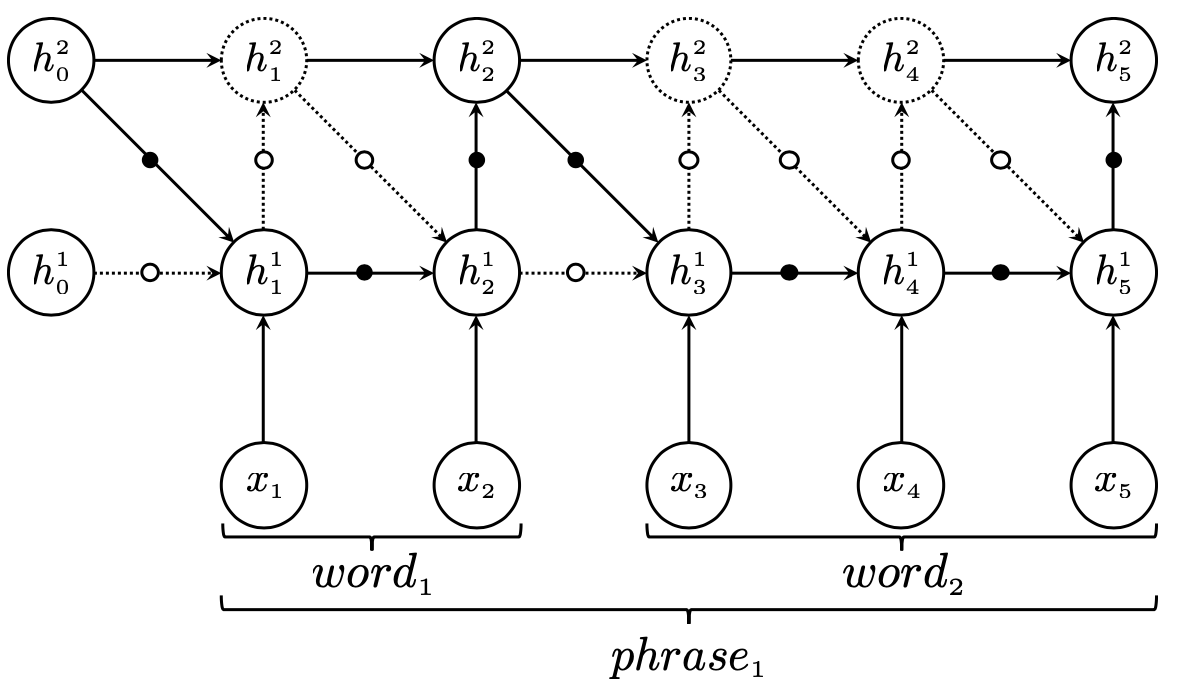
\includegraphics[width=0.55\textwidth]{figures/hmrnn-architecture.png}
        \end{center}
        \caption{Overall Architecture of HMRNN. 
        HM-RNN should learn and discover the structure of the data by itself, textbf{without the use of boundary tokens}. 
        }
        \label{fig:hmrnn-architecture}
    \end{small}
\end{figure}


\subsection{Problem}
The HMRNN addresses the question:
\begin{quote}
    Can an RNN discover hierarchical multiscale structure without explicit hierarchical boundary information?
\end{quote}


\paragraph{Temporal-hierarchical information learning}
Temporal-Hierarchical information exist in many kinds of sequential data, and can easily be explained as a hierarchy of character, word, sentence, and paragraph context. 

\paragraph{Unsupervised boundary detection}
The authors see the unsupervised boundary objective as necessary to learn a temporal-hierarchical information representation from data.
In the past, there have been attempts at setting up a hierarchy of RNNs with the time hierarchies as hyperparameters, 
but allowing the model to learn this unsupervised has advantages:
\begin{enumerate}
    \item The model is robust to variable length words/sentences. 
    \textit{Example:} \texttt{hello} and \texttt{hi} \textit{contain roughly the same word-level information, 
    although one is almost 3 times as long as the other.}
    \item When progressing past a word and sentence-level abstraction, the ground truth information available quickly decreases.
    \textit{Example: Line breaks, paragraph breaks, hyphens, and chapter breaks are very sparsely represented in text datasets.}
\end{enumerate}




\subsection{HMRNN model and components}
The model is summarized in \cref{fig:hmrnn-architecture}.

The HMRNN Model includes a binary boundary detector at each layer, which triggers the different operations. 

\paragraph{COPY, FLUSH, and UPDATE operations} in the HM-RNN are implemented at each abstraction level.

\begin{itemize}
    \item COPY operation copies the state of the current abstraction level to the next cell
    \item UPDATE sparsely nupdates the cell in the next level 
    \item FLUSH happens when a boundary is detected, 
    so the current state representation is ejected to the higher level cell, and the state is reinitialized.
\end{itemize}


\paragraph{Boundary detection gradients and the Slope Annealing Trick} are used with the straight-through estimator, to account for the non-differentiability of the discrete variable. 
Hence, during the backwards pass, the step function used in the forward pass is replaces with a hard sigmoid.
The Slope Annealing trick includes starting the slope of the hard sigmoid as $a=1$ and increasing it during training for the network to slowly learn to pass information through the sigmoid. 


\paragraph{The HM-LSTM} is proposed, as an LSTM model with \(l\in[0...L]\), performing the following update at step $t$ for layer $l$
\begin{equation}\label{eq:hmlstm-update}
     \mathbf{h}^l_t, \mathbf{c}^l_t, z^l_t =
    f^l_{HM-LSTM}(
        \mathbf{c}^l_{t-1}, 
        \mathbf{h}^l_{t-1}, \mathbf{h}^{l-1}_{t}, \mathbf{h}^{l+1}_{t-1},
        z^l_{t-1}, z^{l-t}_t
        )
\end{equation}
with \(f^l_{HM_LSTM}\) being implemented s.t.


\begin{figure}
    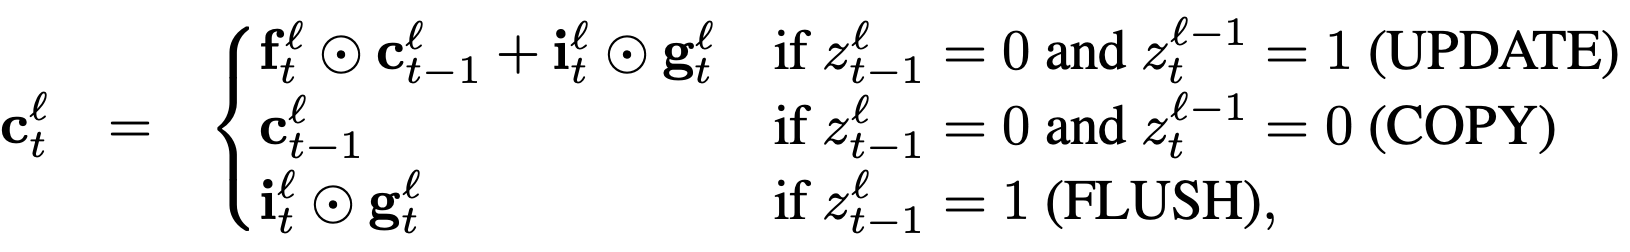
\includegraphics[width=0.45\textwidth]{figures/hmlstm-cell.png}
    \caption{
        HM-LSTM cell state update.
        Here $(f,i,o)$ are gates (forget, input, output) and $g$ is a proposal vector for the cell state.
        }
    \label{eq:hmlstm-cell}
\end{figure}



\paragraph{Model setup for experiments} have the following:
\begin{enumerate}
    \item A continuous input embedding layer
    \item HM-LSTM recurrent unit (3 layers for CL-LM)
    \item Output module of a FFNN, an output embedding layer and a softmax for probability calculation
\end{enumerate}
Here the output module will receive the hidden states of all RNN layers as inputs, adding a gating layer
\begin{equation}
    g^l_t = \mathtt{sigm}(\mathbf{w}^l, [\mathbf{h}^1_t ... \mathbf{h}^L_t])
    \label{eq:hmlstm-output-gate}
\end{equation}
And an output embedding as
\begin{equation}
    \mathbf{h}^e_t = \mathtt{ReLu}
    \left( 
        \sum_{l=1}^L 
        g^l_t
        W^l_t
        \mathbf{h}^l_t   
     \right)
    \label{eq:hmlstm-output-embedding}
\end{equation}



\subsection{Experiments and results}

\paragraph{Character-level language modelling} providing raw text as input, is an ideal task for evaluating raw boundary detection. 
They train the CLLM task using the NLL sequence objective: 
\begin{equation}
    \min_\theta - \frac{1}{N}\sum^N_{n=1}\sum_{t=1}^{T^n} \log p(x^n_t | x^n_{<t}, \theta)
    \label{eq:hmlstm-nll}
\end{equation}

The results on boundary detection are shown in \cref{fig:hmlstm-fun}


\begin{figure}
    \begin{small}
        \begin{center}
            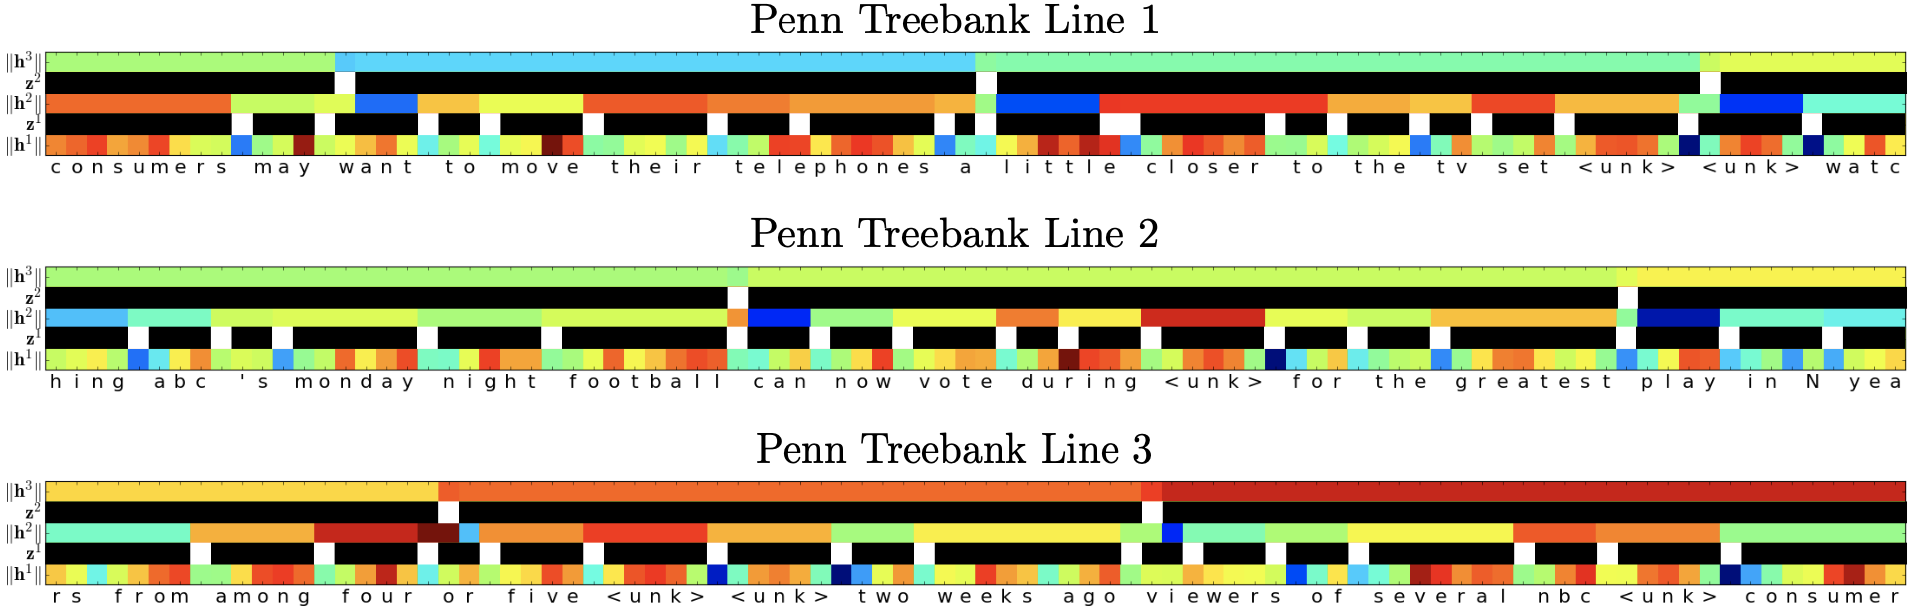
\includegraphics[width=0.95\textwidth]{figures/hmlstm-states.png}
        \end{center}
        \caption{$l^2$ norm of hidden states along with boundary detection states for PTB.l}
        \label{fig:hmlstm-states}
    \end{small}
\end{figure}



